\section{Actividad No 02 – GitLab} 
GitLab nació como un sistema de alojamiento de repositorios Git, es decir, un hosting para proyectos gestionados por el sistema de versiones Git. Sin embargo, alrededor de esta herramienta han surgido muchas otras herramientas muy interesantes para programadores y equipos de desarrollo, que envuelven todo el flujo del desarrollo y el despliegue de aplicaciones, test, etc.
\begin{itemize}

	\item Uso

	GitLab es una herramienta basada en Git, que usas de la misma manera que cualquier otra herramienta similar. Generalmente usas Git a través de la línea de comandos, o a través de programas de interfaz gráfica, o del propio editor de código. Toda esa operativa que ya conoces y que hemos explicado en el Manual de Git, no cambia.

Además del hosting remoto para repositorios GitLab ofrece una interfaz web para controlar el repositorio y muchas otras herramientas. Ofrece la posibilidad de examinar el código en cualquiera de sus versiones, realizar acciones relacionadas con el sistema de repositorios como mergear el código de versiones de proyecto o gestionar las "pull request" (que en GitLab se llaman "merge request"), gestionar problemática de tu software diversa, automatizar procesos como el despliegue o la ejecución de pruebas del software, etc. Toda esta operativa la realizas, o configuras, en GitLab por medio de una web.

	

           \item\textbf{ Funcionalidades}
    
	En GitLab podemos gestionar principalmente proyectos, Grupos y Sinppets. Los proyectos son los protagonistas del sistema, básicamente repositorios de software gestionados por GitLab y todo el ecosistema GitLab. Los grupos son básicamente empresas y usuarios. Los snippets por su parte son como pedazos de código que puedes dejar para hacer cualquier cosa.

Como decimos, dentro de los proyectos es donde se aglutinan la mayoría de las funcionalidades que vamos a resumir:

          \textbf {Overview:}
           Es un listado de todo el proyecto, los archivos, los README.md. Es parecido a lo que vemos cuando accedemos a un proyecto con GitHub. Te da el resumen del repositorio, archivos, commits, etc.

Luego tiene dos subsecciones: En Activity del proyecto te ofrece toda la actividad, de una manera estadística. En Cycle Analytics además te ofrece algo muy novedoso, no disponible en otras herramientas. Básicamente informa el tiempo que se tarda en realizar una funcionalidad, desde que tienes la idea hasta que se incorpora al software, de modo que cualquier persona, incluso sin conocimientos de programación, puede saber el tiempo que ocupó el hacer las tareas. Una información muy valiosa que puede ayudar a futuro a estimar mejor el tiempo de trabajo necesario para nuevas funcionalidades. Obviamente, cuantas más issues tengas en el sistema, más datos tendrás para saber el tiempo que necesitas para las próximas tareas.

           \textbf {Repository:}
Dentro de la sección "Repository" tenemos varias opciones diversas que afectan al repositorio del proyecto.

Tenemos "Files", donde se puede navegar por los directorios y archivos, cuyo código podemos ver, e incluso editar los ficheros. Está disponible una visualización por ramas y dispone de utilidades diversas para poder hacer cosas relacionadas con el repositorio remoto, ahorrando la necesidad de lanzar comandos. Tiene un buscador de archivos muy potente.


           \textbf {Issues:}
Este es otra de las grandes utilidades de GitLab, que permite definir cualquier problema que se detecta en el software y darle seguimiento. Seguro que las conocemos porque es una de las partes fundamentales de GitHub y habremos navegado por ellas en decenas de ocasiones.

Básicamente nos permite ver las issues generadas en un proyecto, mantener discusiones sobre ellas, y controlar los flujos de trabajo para su resolución, permitiendo definir las personas que deben resolverla, el tiempo estimado y el usado, la fecha límite, el peso de las tareas, etc.

      

	\begin{center}
	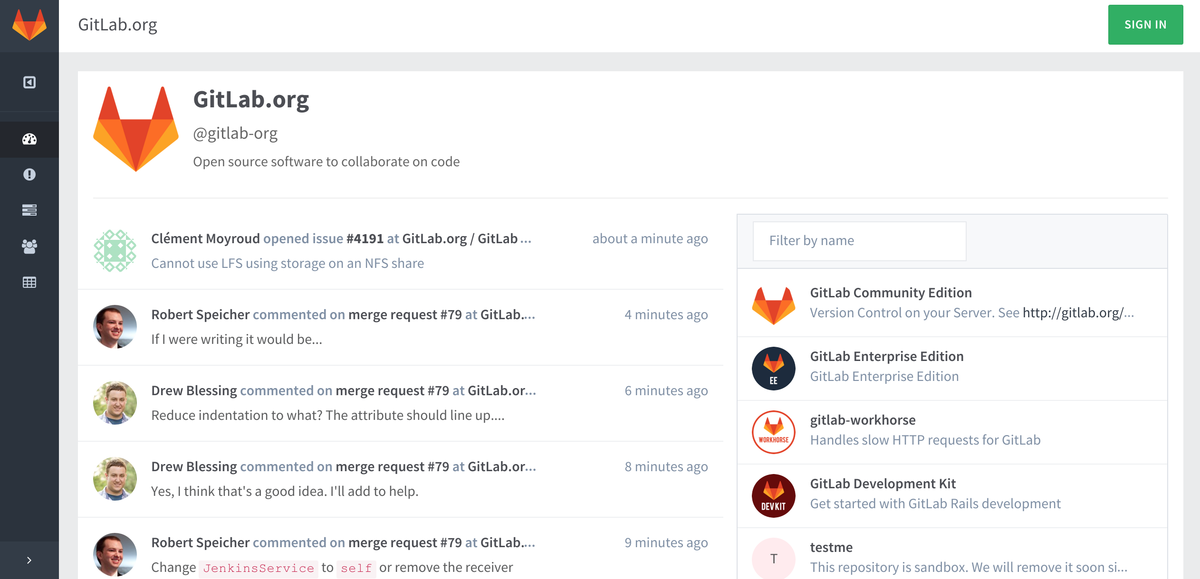
\includegraphics[width=17cm]{./Imagenes/image3} 
	\end{center}


\end{itemize} 